\documentclass[12pt]{article}
\usepackage[a4paper]{geometry}
\usepackage[utf8]{inputenc}
\usepackage{fancyhdr}
\usepackage{lastpage}
\usepackage{graphicx, wrapfig, subcaption, setspace, booktabs}
\usepackage{graphicx}
\usepackage[T1]{fontenc}
\usepackage[font=small, labelfont=bf]{caption}
\usepackage[protrusion=true, expansion=true]{microtype}
\usepackage[english]{babel}
\usepackage{sectsty}
\usepackage{url, lipsum}
\usepackage[T1]{fontenc}
\usepackage{icomma}
\usepackage{siunitx}
\usepackage{ragged2e}
\usepackage{amsmath}
\usepackage{comment}
\usepackage{enumerate}
\usepackage{anysize}

\newcommand{\HRule}[1]{\rule{\linewidth}{#1}}
\onehalfspacing
\setcounter{tocdepth}{5}
\setcounter{secnumdepth}{5}

\begin{document}

\begin{titlepage}

\title{ \normalsize 
        \begin{center}
        
\includegraphics[height=6cm]{Logo.jpg}
        \end{center}
        \LARGE \textsc{\textbf{Universidad De Sonora}} \\ \bigskip
		\Large División de Ciencias Exactas y Naturales \\
        Licenciatura En Física \\ \bigskip
        \bigskip
        Física Computacional I
		\\ [0.1cm]  
		\HRule{2pt} \\
		\Large \textbf{{Reporte de Actividad 10}} \\
        \textit{\textbf{"Teoría del Caos y el Mapeo Logístico"}}
		\HRule{2pt} \\
		\normalsize \vspace*{0.001\baselineskip}}
        
\date{\bigskip \Large Hermosillo, Sonora  \hspace*{\fill}  Mayo 16 de 2018}

        
\author{
		\Large\textbf{ César Omar Ramírez Álvarez} \\ \bigskip
        \\ \bigskip
       \Large Profr. Carlos Lizárraga Celaya}
       \end{titlepage}
       \maketitle
       

\newpage
\pagestyle{plain}
\section*{Introducción}
El presente informe es producto de la décima práctica de la materia de Física Computacional I, en esta ocasión se analizará un artículo de Geoff Boeing acerca de la Teoría del Caos y el Mapeo Logístico utilizando Python. Cabe resaltar, que solamente se utilizó la información presentada en l blog, ya que la reproducción de las gráficas por nuestro lado fue realizada con el Sistema de Álgebra Computacional llamado wxMaxima.\\

Entonces, a continuación se presentará una breve síntesis del blog de Geoff Boeing, en donden se mencionan sobre ciertas caracteristicas de los sistemas no lineales dinámicos y sobre los sistemas caóticos, fundamentandose en la idea del crecimiento poblacional por distintas generaciones. Como apoyo visual se presentarán las gráficas generadas en el sistema de álgebra computacional donde se ve claramente en que consisten dichos fenómenos.

\section*{Síntesis (Teoría del Caos y el Mapeo Logístico)}

La teoría del caos es una rama de las matemáticas que se ocupa de los sistemas dinámicos no lineales. Un sistema es solo un conjunto de componentes interactivos que forman un todo más grande. No lineal significa que, debido a la retroalimentación o los efectos multiplicativos entre los componentes, el todo se convierte en algo más que simplemente sumar las partes individuales. Por último, dinámico significa que el sistema cambia con el tiempo en función de su estado actual.\\

Los sistemas caóticos son un sub-tipo simple de sistemas dinámicos no lineales. Pueden contener muy pocas partes interactuantes y éstas pueden seguir reglas muy simples, pero todos estos sistemas tienen una dependencia muy sensible de sus condiciones iniciales. A pesar de su simplicidad determinista, con el tiempo estos sistemas pueden producir un comportamiento totalmente impredecible y tremendamente divergente (también conocido como caótico). Edward Lorenz, el padre de la teoría del caos,  describió el caos como "cuando el presente determina el futuro, pero el presente aproximado no determina aproximadamente el futuro".

\subsection*{El Mapa Logístico}

Este modelo se basa en la función logística común de curva en forma de $S$  que muestra cómo una población crece lentamente, luego rápidamente, antes de disminuir a medida que alcanza su capacidad de carga. La función logística utiliza una ecuación diferencial que trata el tiempo como continuo. En su lugar, el mapa de logística utiliza una ecuación de diferencia no lineal para observar los pasos de tiempo discretos. Se llama mapa logístico  porque asigna el valor de la población en cualquier paso de tiempo a su valor en el siguiente paso:

$$x_{t+1}=rx_t(1-x_t)$$

Esta ecuación define las reglas o dinámicas de nuestro sistema: $x$ representa la población en cualquier momento dado  $t$, y $r$ representa la tasa de crecimiento. En otras palabras, el nivel de población en cualquier momento dado es una función del parámetro de tasa de crecimiento y el nivel de población del paso de tiempo anterior. Si la tasa de crecimiento es demasiado baja, la población morirá y se extinguirá. Mayores tasas de crecimiento podrían establecerse hacia un valor estable o fluctuar a través de una serie de auges y caídas de la población.

\subsection*{Comportamiento del Sistema y Atractores}

Se presenta una gráfica donde se muestran generaciones de poblaciones con distintas tazas de crecimiento:

\begin{center}
    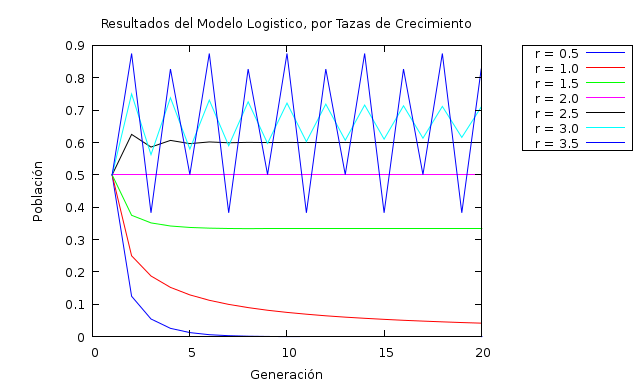
\includegraphics[height=9cm]{Primera.png}
\end{center}

Aquí puede ver fácilmente cómo cambia la población a lo largo del tiempo, dadas las diferentes tasas de crecimiento. La línea azul representa una tasa de crecimiento de 0.5, y rápidamente cae a cero. La población muere. La línea cian representa una tasa de crecimiento de 2.0 y se mantiene estable a un nivel de población de 0.5. Las tasas de crecimiento de 3.0 y 3.5 son más interesantes. Mientras que la línea amarilla para 3.0 parece estar convergiendo lentamente hacia un valor estable, la línea gris para 3.5 solo parece rebotar.\\

Un atractor es el valor, o conjunto de valores, con los que el sistema se establece a lo largo del tiempo. Cuando el parámetro de tasa de crecimiento se establece en 0.5, el sistema tiene un atractor de punto fijo en el nivel de población 0 como se muestra en la línea azul.\\

Un sistema caótico tiene un atractor extraño , alrededor del cual el sistema oscila para siempre, nunca se repite o se establece en un estado estable de comportamiento. Nunca golpea el mismo punto dos veces y su estructura tiene una forma fractal, lo que significa que existen los mismos patrones en todas las escalas, sin importar cuánto se acerque a ella.

\subsection*{Bifurcaciones y el Camino al Caos}

Para mostrar esto más claramente, ejecutemos nuevamente el modelo logístico, esta vez para 200 generaciones en 1,000 tasas de crecimiento entre 0.0 y 4.0. Cuando produjimos el gráfico de líneas de arriba, tuvimos solo 7 tasas de crecimiento. Esta vez tendremos 1,000, así que tendremos que visualizarlo de una manera diferente, usando algo llamado diagrama de bifurcación:
\begin{center}
    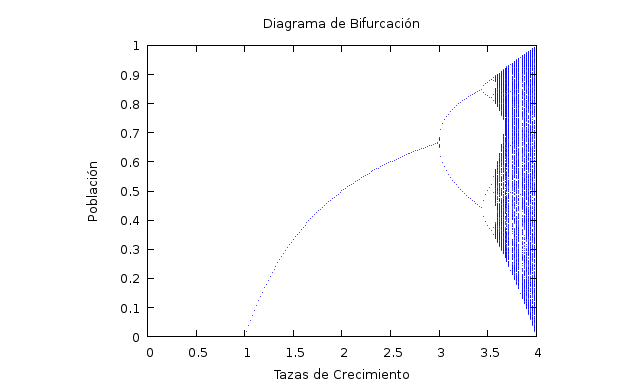
\includegraphics[height=8cm]{Segunda.png}
\end{center}

Cada sector vertical representa los valores de población a los que se dirige el mapa logístico para ese valor de parámetro. En otras palabras, la porción vertical sobre cada tasa de crecimiento es el atractor de la tasa de crecimiento.\\

Para tasas de crecimiento inferiores a 1.0, el sistema siempre colapsa a cero (extinción). Para tasas de crecimiento entre 1.0 y 3.0, el sistema siempre se establece en un nivel de población exacto y estable. Mire la porción vertical por encima de la tasa de crecimiento 2.5\\
Solo hay un valor de población representado (0.6) y corresponde al lugar donde se asienta la línea magenta en el gráfico de líneas mostrado anteriormente. Nunca se instala en un punto fijo o un ciclo límite.

Entonces, ¿por qué se llama esto un diagrama de bifurcación?
\begin{center}
    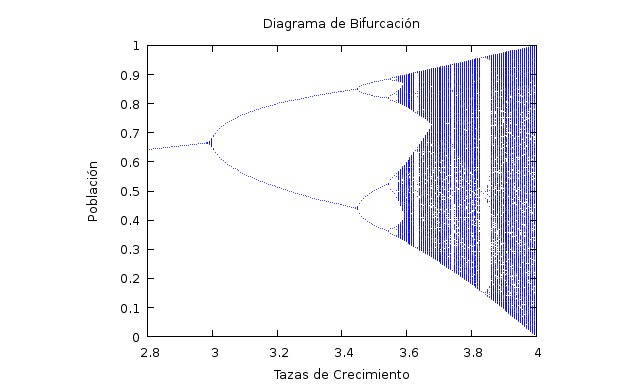
\includegraphics[height=8cm]{Tercera.png}
\end{center}

En el corte vertical por encima de la tasa de crecimiento 3.0, los valores de población posibles se bifurcan en dos caminos discretos. Con la tasa de crecimiento 3.2, el sistema oscila esencialmente entre dos valores de población: uno alrededor de 0.5 y otro alrededor de 0.8. En otras palabras, a esa tasa de crecimiento, aplicar la ecuación logística a uno de estos valores produce el otro.

\subsection*{El Comienzo del Caos}

Más allá de una tasa de crecimiento de 3.6, las bifurcaciones aumentan hasta que el sistema es capaz eventualmente de aterrizar en  cualquier valor de población. Esto se conoce como el camino que duplica el período al caos. A medida que ajusta el parámetro de la tasa de crecimiento hacia arriba, el mapa logístico oscilará entre 2, luego 4, luego 8, luego 16, y luego 32 (y así sucesivamente) los valores de población. Estos son períodos , al igual que el período de un péndulo.\\
 
 Para cuando alcanzamos la tasa de crecimiento 3.9, se ha bifurcado tantas veces que el sistema ahora salta, aparentemente de forma aleatoria, entre todos los valores poblacionales. Solo digo aparentemente de forma aleatoria porque definitivamente no es  aleatorio. Por el contrario, este modelo sigue reglas deterministas muy simples pero produce aparente aleatoriedad. Esto es caos: determinista y aperiódico.\\

Hagamos zoom de nuevo, a la estrecha porción de tasas de crecimiento entre 3.7 y 3.9:
\begin{center}
    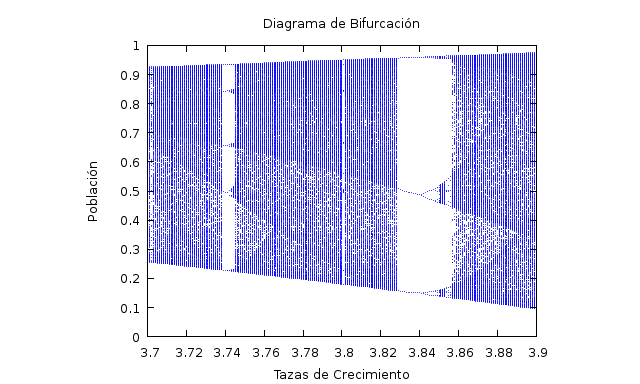
\includegraphics[height=8cm]{Cuarta.png}
\end{center}
Al acercarnos, comenzamos a ver la belleza del caos. Del ruido emergen extraños patrones y umbrales de turbulencias a cada lado del cual el sistema se comporta de manera muy diferente. Entre los parámetros de tasa de crecimiento de 3.82 y 3.84, el sistema pasa del caos nuevamente al orden, oscilando entre solo tres valores de población (aproximadamente 0.15, 0.55 y 0.95). Pero luego se bifurca nuevamente y vuelve al caos a tasas de crecimiento superiores a 3.86.

\subsection*{Fractales y Extraños Atractores}
En el gráfico anterior, las bifurcaciones en torno a la tasa de crecimiento 3.85 parecen un poco familiares. Vamos a acercarnos al centro:

\begin{center}
    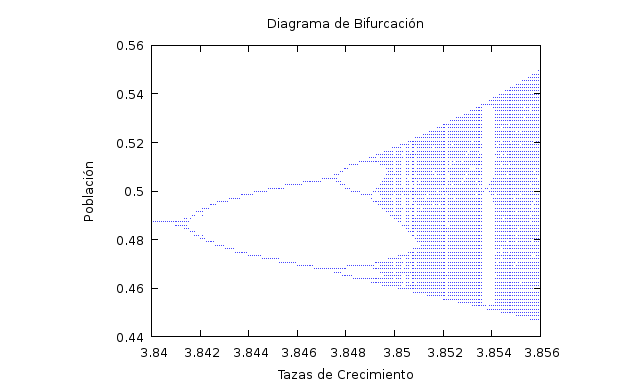
\includegraphics[height=8cm]{Quinta.png}
\end{center}
Increíblemente, vemos la misma estructura exacta que vimos anteriormente en el nivel macro. De hecho, si seguimos haciendo zoom infinitamente en esta trama, seguiremos viendo la misma estructura y patrones a escalas cada vez más finas, para siempre. \\

 Los fractales son auto-similares , lo que significa que tienen la misma estructura en todas las escalas. Al acercarse a ellos, encontrará copias más pequeñas de la macroestructura más grande. \\
 
 Otra forma de visualizar esto es con un diagrama de fase  (o  diagrama de Poincaré ), que traza el valor de la población en la generación  $t + 1$ en el eje y contra el valor de la población en $t$ en el eje $x$. Profundizo en diagramas de fases animadas , tridimensionales y tridimensionales con mayor detalle en una publicación posterior.\\
 
 Recordando que nuestro modelo sigue una regla determinista simple, por lo que si conocemos el valor poblacional de una determinada generación, podemos determinar fácilmente el valor de la siguiente generación:
 \begin{center}
    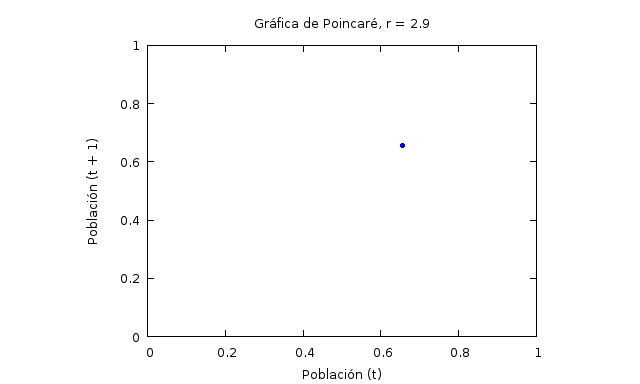
\includegraphics[height=4.5cm]{Sexta.png} \hspace*{\fill}  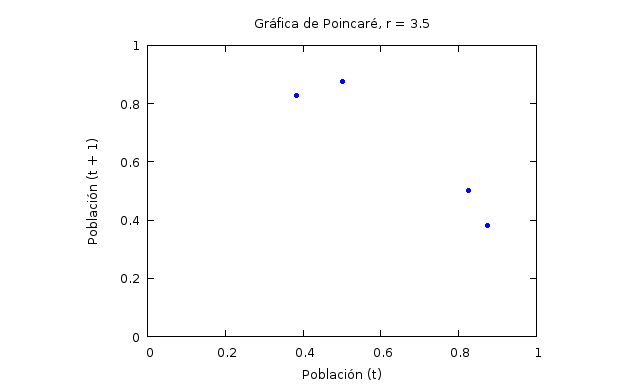
\includegraphics[height=4.5cm]{Septima.png}
\end{center}
El diagrama de fase de arriba a la izquierda muestra que el mapa logístico se dirige hacia un atractor de punto fijo en 0.655 (en ambos ejes) cuando el parámetro de tasa de crecimiento se establece en 2.9. Esto corresponde a la porción vertical por encima del valor del eje x de 2.9 en los diagramas de bifurcación que se muestran anteriormente. La gráfica de la derecha muestra un atractor de ciclo límite. Cuando la tasa de crecimiento se establece en 3.5, el mapa logístico oscila en cuatro puntos, como se muestra en este diagrama de fases (y en los diagramas de bifurcación de antes).\\

Esto es lo que sucede cuando estas bifurcaciones que duplican el período conducen al caos:
\begin{center}
    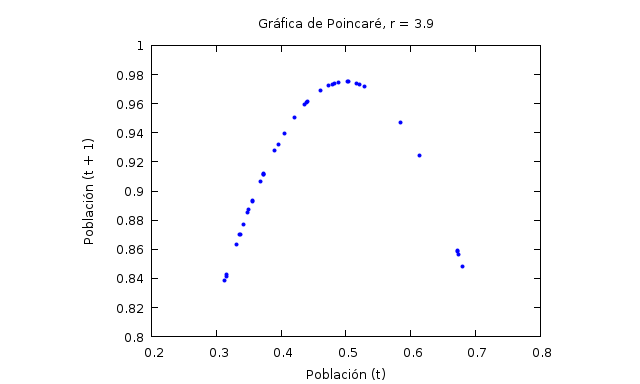
\includegraphics[height=4.5cm]{Octava.png} \hspace*{\fill}  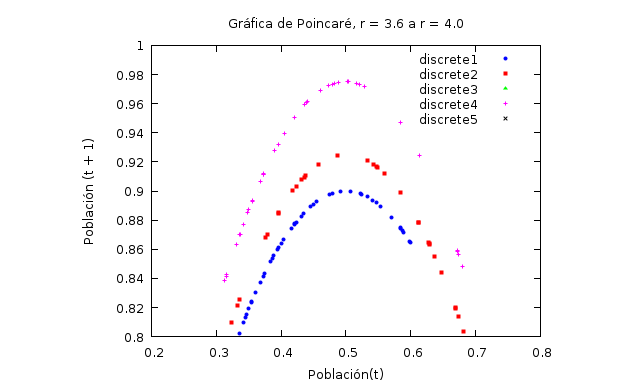
\includegraphics[height=4.5cm]{Novena.png}
\end{center}
La gráfica de la izquierda muestra una parábola formada por un parámetro de tasa de crecimiento de 3.9. La gráfica de la derecha muestra 50 parámetros diferentes de tasa de crecimiento entre 3.6 y 4.0. Este rango de parámetros representa el régimen caótico: el rango de valores de parámetros en los que el mapa logístico se comporta de manera caótica. Cada tasa de crecimiento forma su propia curva. Estas parábolas nunca se superponen, debido a su geometría fractal y la naturaleza determinista de la ecuación logística.
\subsection*{Caos vs Aleatoriedad}
Estos diagramas de fase representan el espacio de estado bidimensional : un espacio imaginario que usa variables del sistema como sus dimensiones. Cada punto en el espacio de estado es un posible estado del sistema, o en otras palabras, un conjunto de valores variables.\\

De hecho, puede ser difícil determinar si ciertas series de tiempo son caóticas o simplemente aleatorias cuando no se comprende por completo su dinámica subyacente. Tomemos estos dos como ejemplo:
\begin{center}
    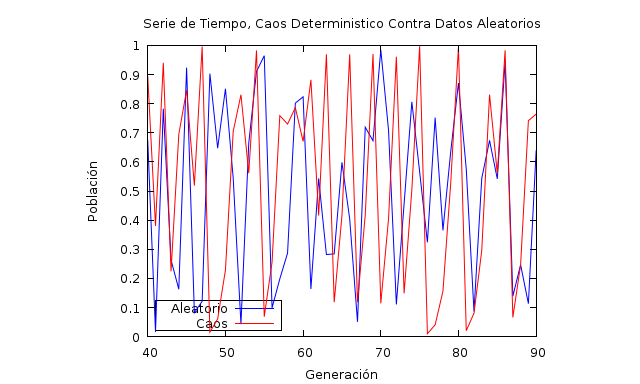
\includegraphics[height=8cm]{Decima.png}
\end{center}
Ambas líneas parecen saltar al azar. La línea azul no representan datos aleatorios, pero la línea roja viene de nuestro modelo logístico cuando la tasa de crecimiento se establece en 3,99. Este es un caos determinista, pero es difícil diferenciarlo de la aleatoriedad. Entonces, visualicemos estos mismos dos conjuntos de datos con un diagrama de fase en lugar de gráficos de líneas:
\begin{center}
    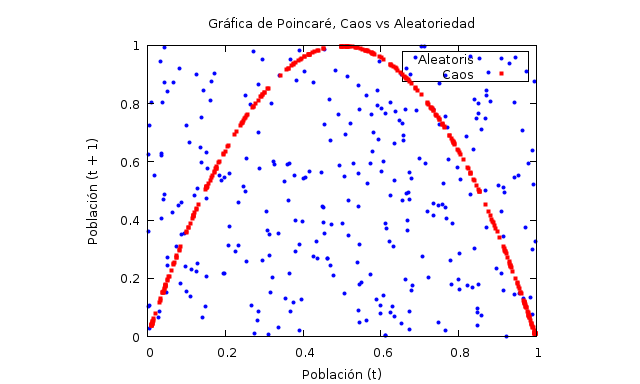
\includegraphics[height=8cm]{Onceava.png}
\end{center}
Ahora podemos ver nuestro sistema caótico (en rojo, arriba) limitado por su atractor extraño. Por el contrario, los datos aleatorios (en azul, arriba) solo parecen ruido.
\subsection*{El Efecto Mariposa}
Los sistemas caóticos también se caracterizan por su dependencia sensible de las condiciones iniciales. No tienen una cuenca de atracción que recolecte puntos cercanos a lo largo del tiempo en un atractor de ciclo de punto fijo o límite. Por el contrario, con un atractor extraño, los puntos cercanos divergen con el tiempo.\\

Esto dificulta el modelado y la predicción del mundo real, ya que debe medir los parámetros y el estado del sistema con una precisión infinita. De lo contrario, pequeños errores en la medición o el redondeo se combinan con el tiempo hasta que el sistema se desconecta drásticamente. Fue a través de uno de esos  errores de redondeo que Lorenz descubrió el caos por primera vez. Recuerde sus palabras al principio de esta pieza: "el presente determina el futuro, pero el presente aproximado no determina aproximadamente el futuro".\\

Como ejemplo de esto, ejecutemos el modelo logístico con dos valores de población iniciales muy similares:

\begin{center}
    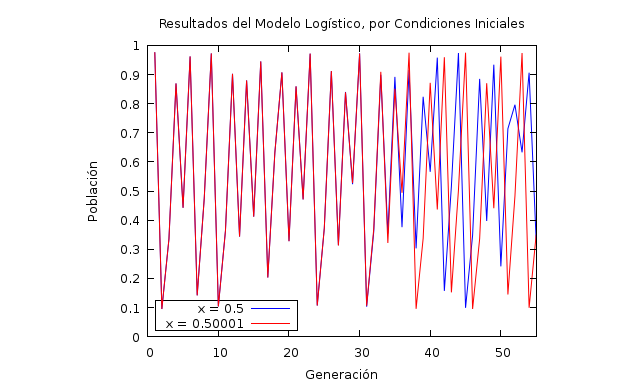
\includegraphics[height=8cm]{Doceava.png}
\end{center}

Ambos tienen el mismo parámetro de tasa de crecimiento, 3.9. La línea azul representa un valor poblacional inicial de 0.5. La línea roja representa una población inicial de 0.50001. Estas dos condiciones iniciales son extremadamente  similares entre sí. En consecuencia, sus resultados parecen esencialmente idénticos para las primeras 30 generaciones. Después de eso, sin embargo, la minúscula diferencia en las condiciones iniciales comienza a complicarse. Para la generación 40, las dos líneas muestran poco en común.\\

Esto es famoso por el efecto mariposa : una mariposa bate sus alas en China y provoca un tornado en Texas. Pequeños eventos compuestos e irreversiblemente alteran el futuro del universo. En el gráfico de líneas de arriba, una pequeña fluctuación de 0.00001 hace una enorme diferencia en el comportamiento y el estado del sistema 50 generaciones más tarde.

\subsection*{Las Implicaciones del Caos}
Los sistemas caóticos y fractales del mundo real incluyen grifos con fugas , helechos , frecuencias cardíacas y generadores de números aleatorios . Muchos estudiosos han estudiado las implicaciones de la teoría del caos para las ciencias sociales , las ciudades y la planificación urbana . El caos indica fundamentalmente que existen límites para el conocimiento y la predicción. Algunos futuros pueden ser desconocidos con precisión. Los sistemas deterministas pueden producir un comportamiento salvajemente fluctuante y no repetitivo. Las intervenciones en un sistema pueden tener resultados impredecibles, incluso si inicialmente cambian las cosas solo ligeramente, ya que estos efectos se combinan con el tiempo.

\section*{Conclusión}
El hecho de utilizar wxMaxima para hacer esta práctica, queda demostrado el poder que tienen este tipo de sistemas algebraicos computacionales, ya que con ciertas dificultades (por motivos de tiempos y pcoco conocimiento del funcionamiento) pero se logró reproducir los gráficos que estaban realizados en Python por lo que considerouna muy buena herramienta a el software wxMaxima.\\

Por otro lado, el tema que se trato me parecio mu interesante y muy buena ejemplificación, a parte de uqe se tuvo una visualización para el mejor entendimiento. Sin duda wxMaxima será de gran apoyo durante la licenciatura y todo lo que resta. Muy buena actividad, digna del cierre de la asignatura.

\newpage

\section*{Bibliografía}
\begin{itemize}
\item  Chaos Theory and the Logistic Map - Geoff Boeing. (2018). Recuperado desde:\\ http://geoffboeing.com/2015/03/chaos-theory-logistic-map/

\item Chaotic dynamics with Maxima. (2018). Recuperado desde:\\ https://arxiv.org/pdf/1301.3240.pdf

\item Logistic map. (2018). Recuperado desde:\\ https://en.wikipedia.org/wiki/Logistic\_map

\item Diagrama de bifurcación. (2018). Recuperado desde:\\ https://es.wikipedia.org/wiki/Diagrama\_de\_bifurcaci\%C3\%B3n
\end{itemize}

\end{document}



